\section{Results}\label{sec:results}
In this section, we describe the results of our experiment. 

\begin{figure*}[t!]
    \centering
    \subfigure[North American resolvers]{%
        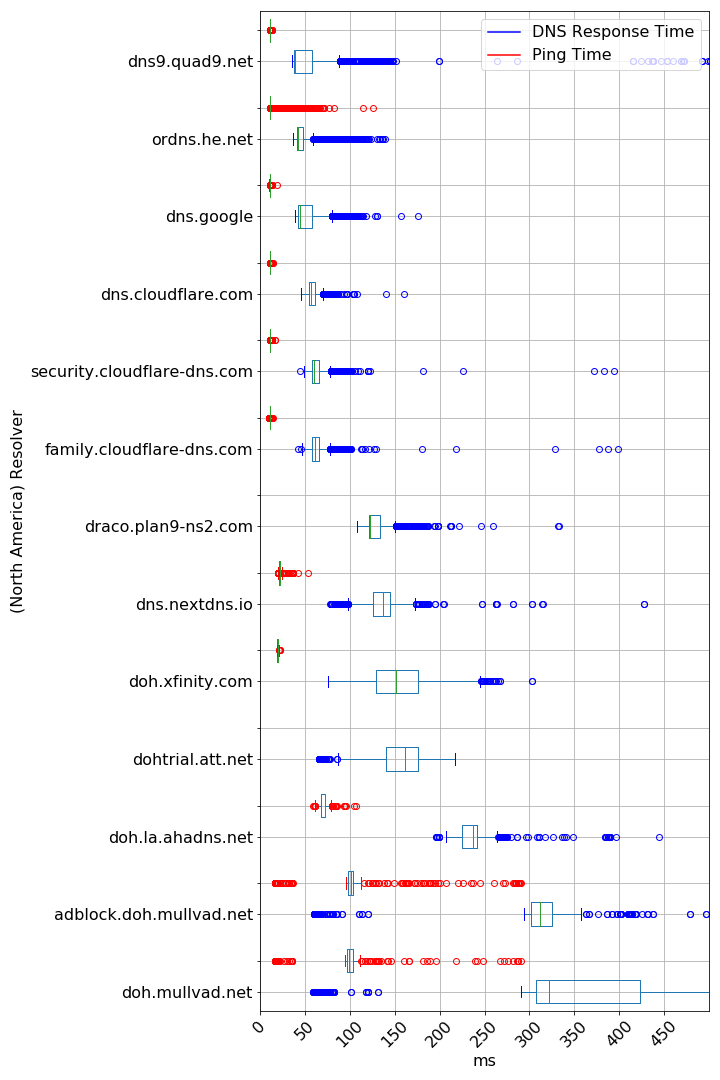
\includegraphics[width=0.5\textwidth]{figures/Ohio_North_America.png}
    }
    \subfigure[Asian resolvers]{%
        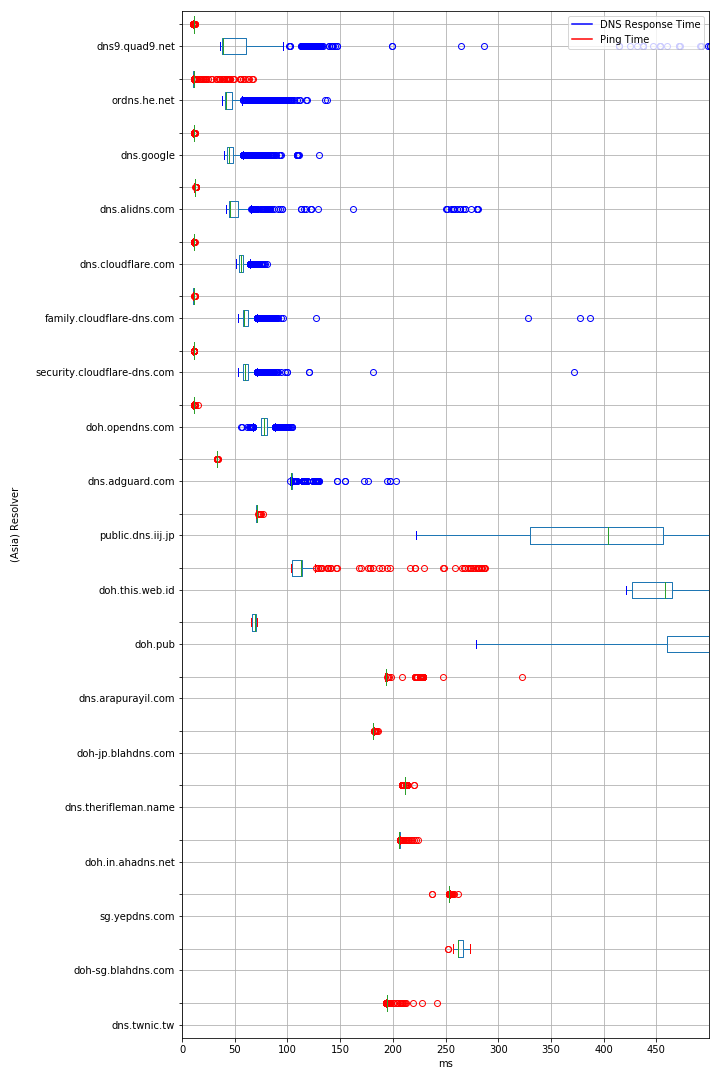
\includegraphics[width=0.5\textwidth]{figures/Ohio_Asia.png}
    }
    \subfigure[European resolvers]{%
        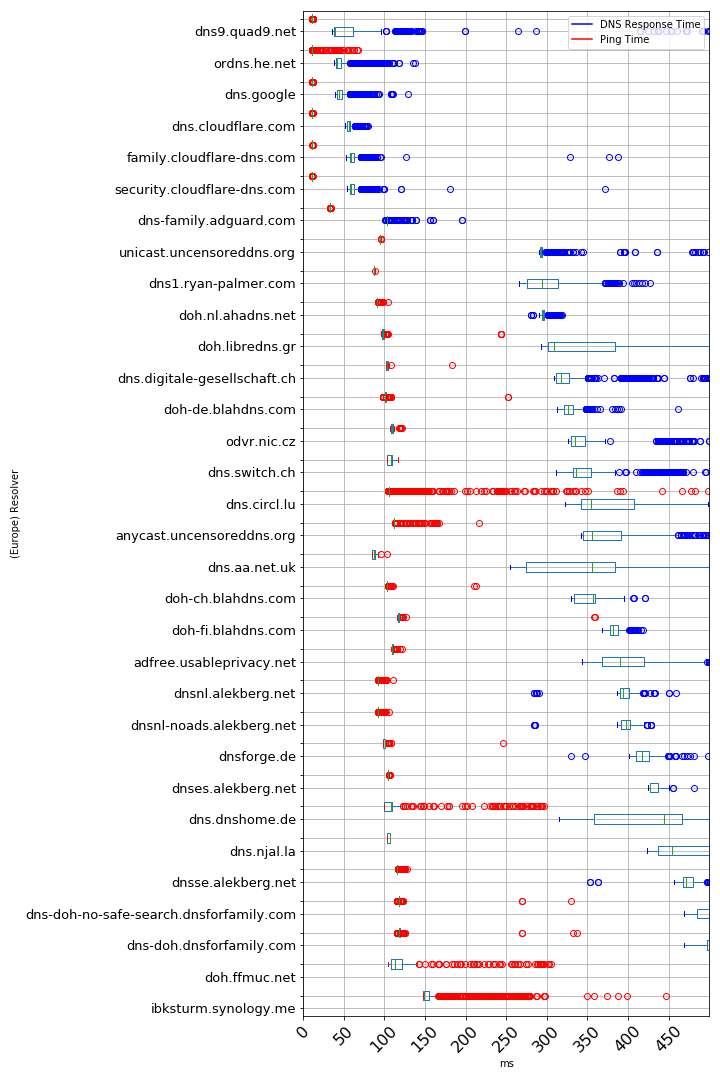
\includegraphics[width=0.5\textwidth]{figures/Ohio_Europe.png}
    }
    \caption{Box-plots of resolvers measured from a vantage point in Ohio, USA}
\end{figure*}

\begin{figure*}[t!]
    \centering
    \subfigure[North American resolvers]{%
        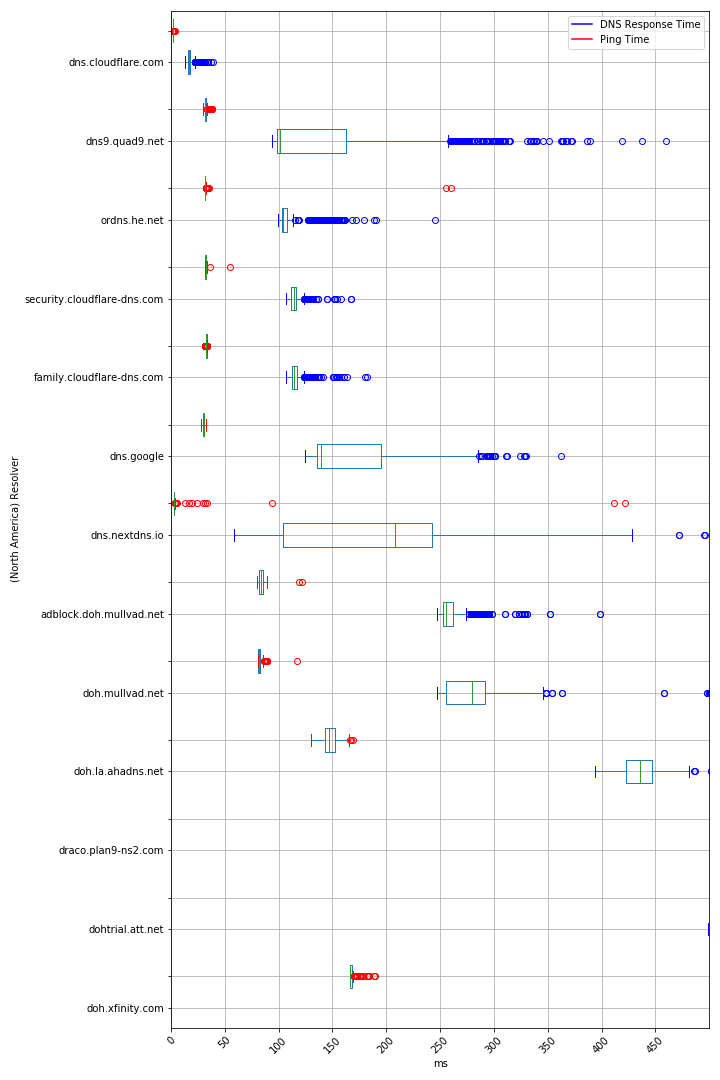
\includegraphics[width=0.5\textwidth]{figures/Seoul_North_America.png}
    }
    \subfigure[Asian resolvers]{%
        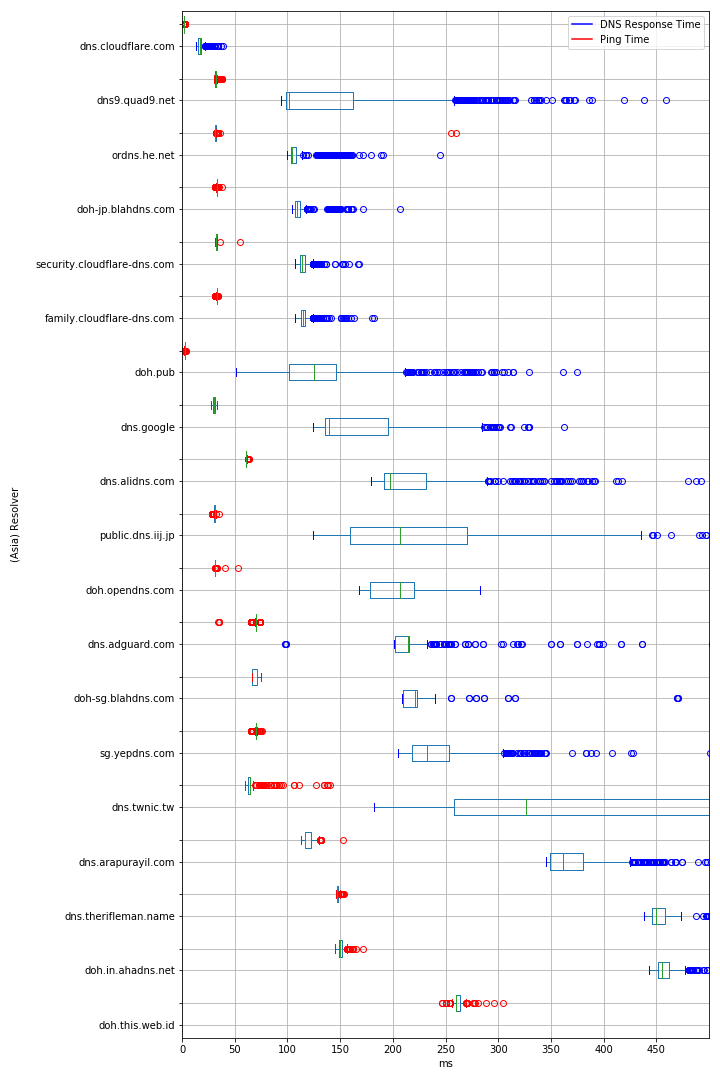
\includegraphics[width=0.5\textwidth]{figures/Seoul_Asia.png}
    }
    \subfigure[European resolvers]{%
        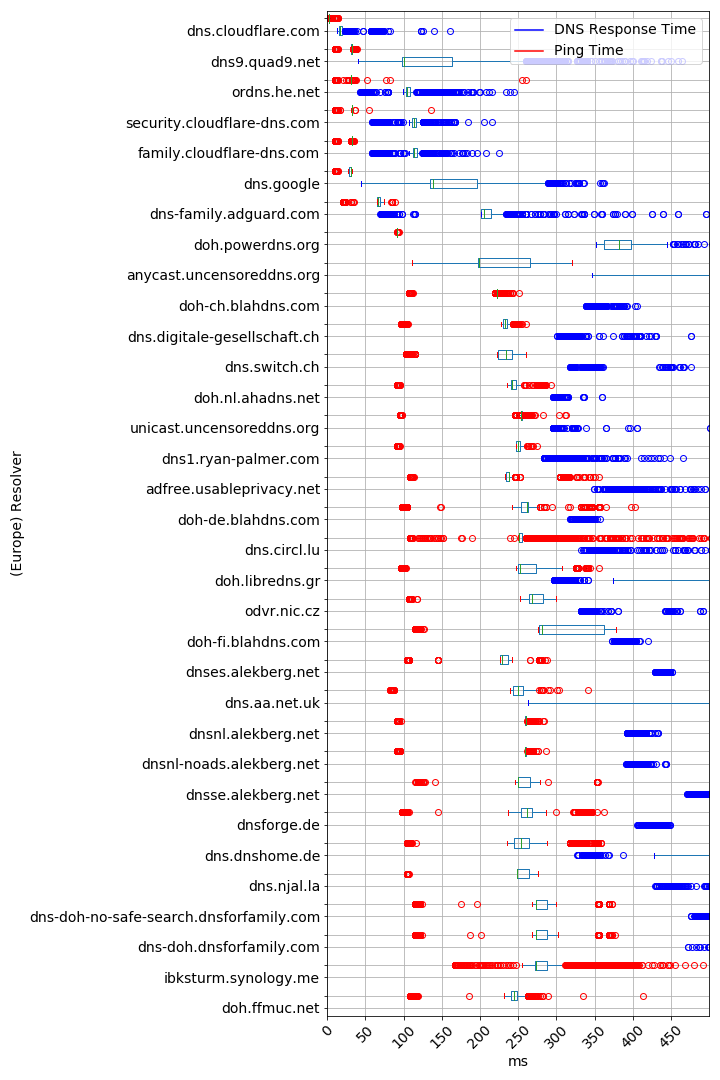
\includegraphics[width=0.5\textwidth]{figures/Seoul_Europe.png}
    }
    \caption{Box-plots of resolvers measured from a vantage point in Seoul, South Korea}
\end{figure*}

\begin{figure*}[t!]
    \centering
    \subfigure[North American resolvers]{%
        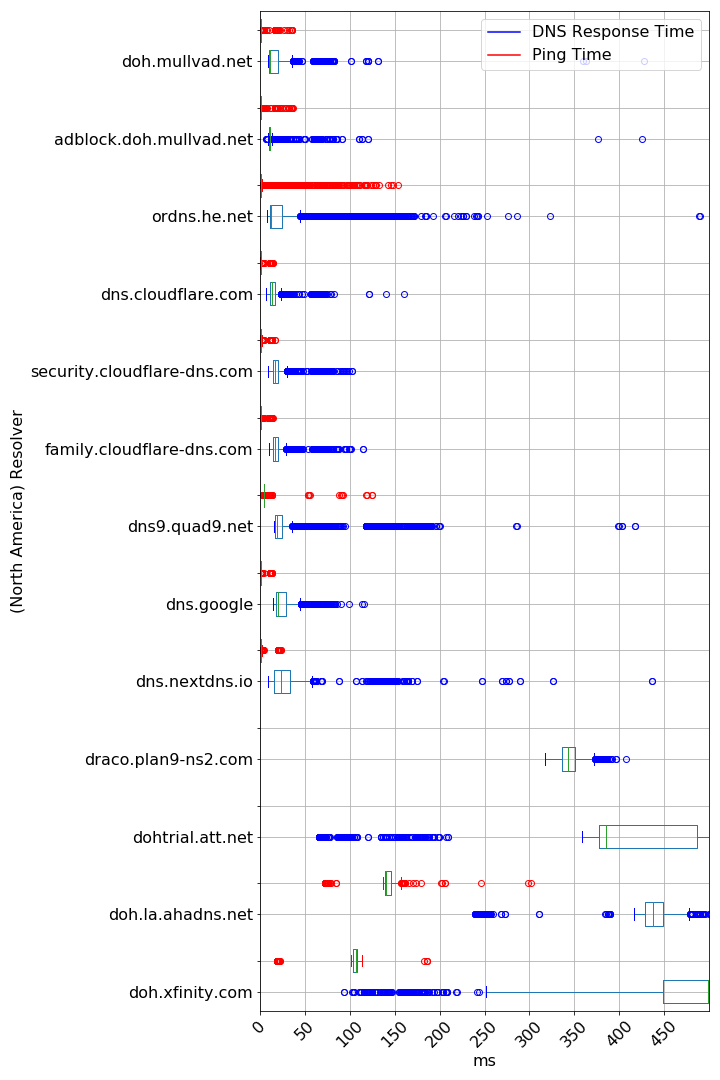
\includegraphics[width=0.5\textwidth]{figures/Frankfurt_North_America.png}
    }
    \subfigure[Asian resolvers]{%
        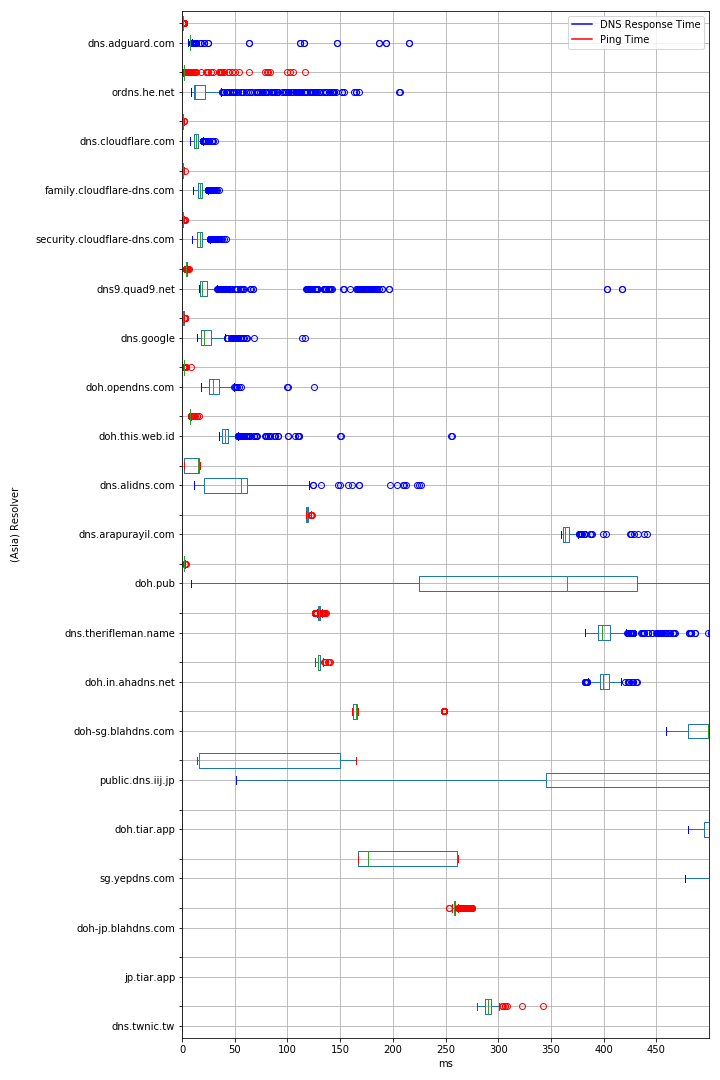
\includegraphics[width=0.5\textwidth]{figures/Frankfurt_Asia.png}
    }
    \subfigure[European resolvers]{%
        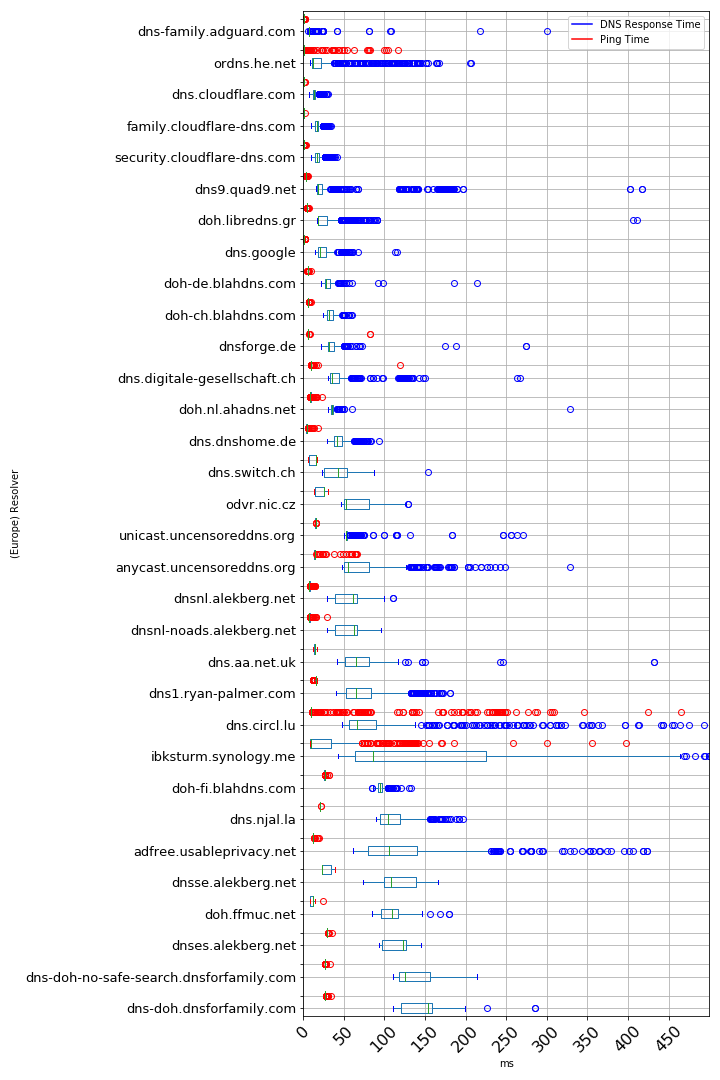
\includegraphics[width=0.5\textwidth]{figures/Frankfurt_Europe.png}
    }
    \caption{Box-plots of resolvers measured from a vantage point in Frankfurt, Germany}
\end{figure*}

\begin{figure*}[t!]
    \centering
    \subfigure[North American resolvers]{%
        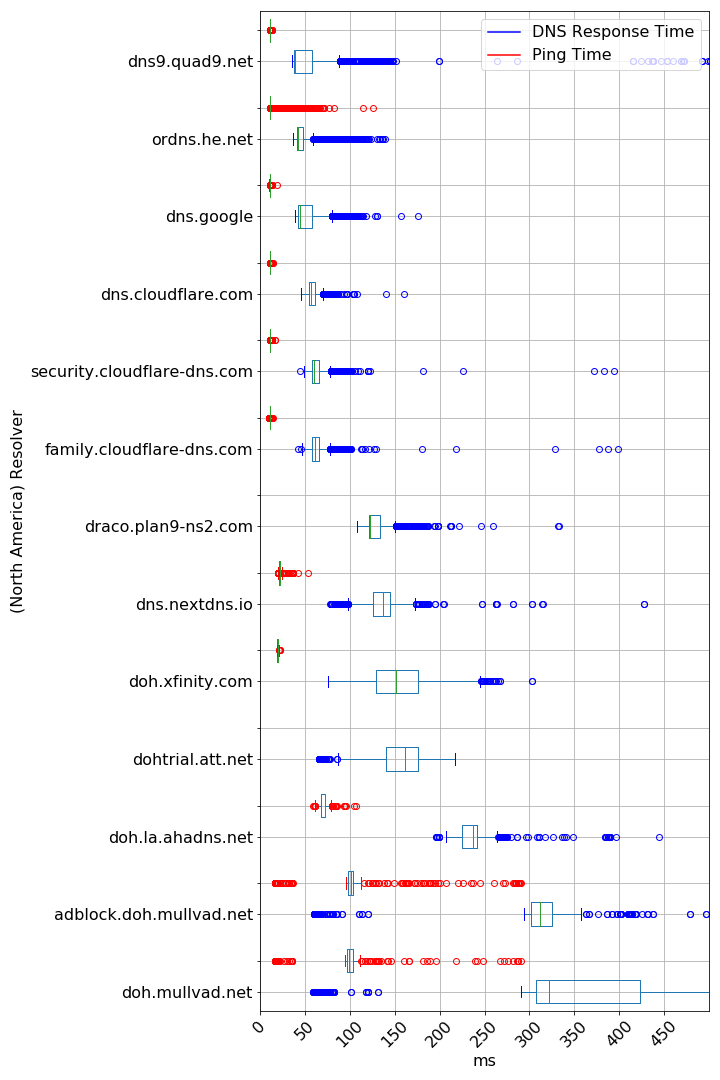
\includegraphics[width=0.5\textwidth]{figures/Ohio_North_America.png}
    }
    \subfigure[Asian resolvers]{%
        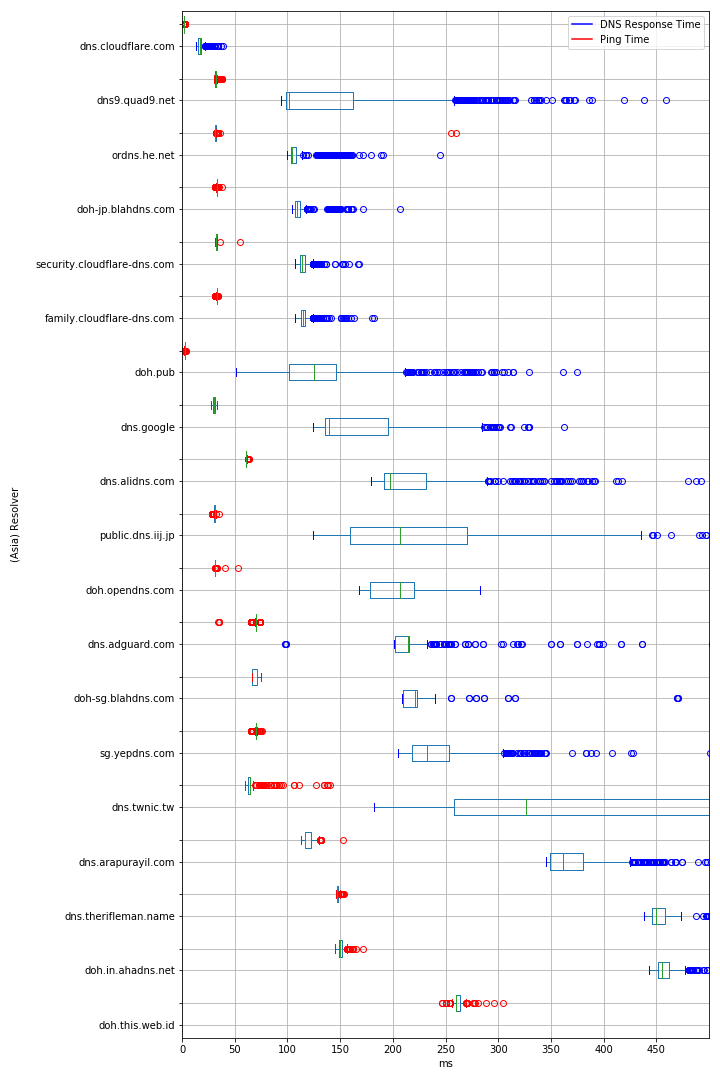
\includegraphics[width=0.5\textwidth]{figures/Seoul_Asia.png}
    }
    \subfigure[European resolvers]{%
        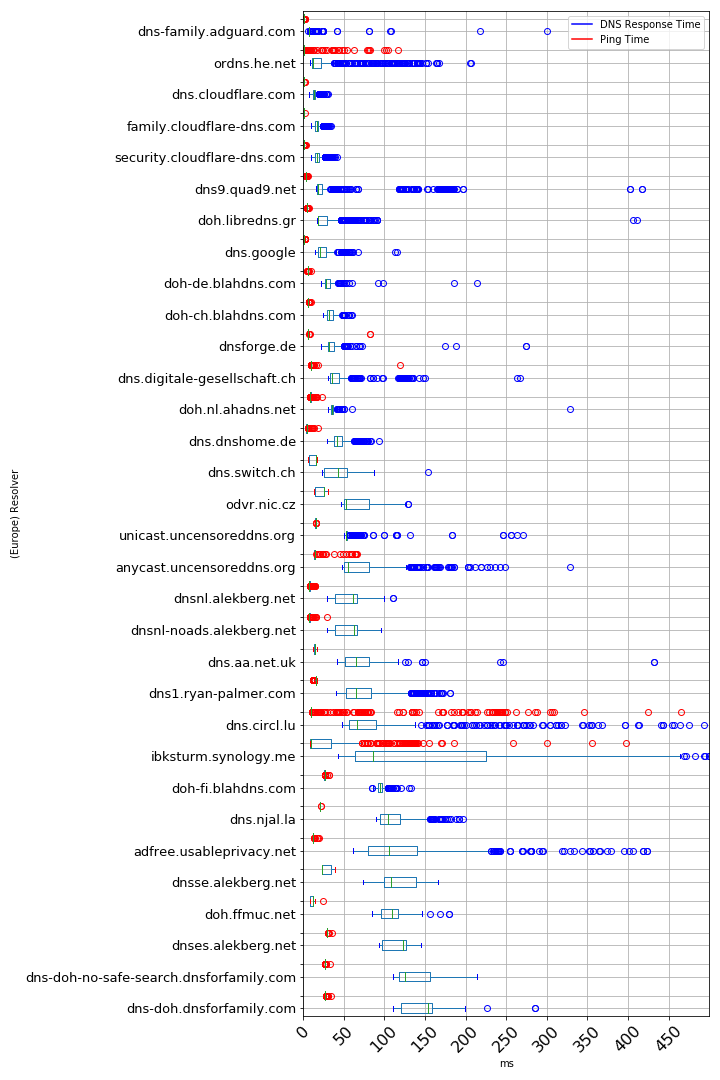
\includegraphics[width=0.5\textwidth]{figures/Frankfurt_Europe.png}
    }
    \caption{Comparing local to local}
\end{figure*}

\begin{table}
\centering
\begin{tabular}{lllll}
\hline
\textbf{Location} & \textbf{Resolver} & \textbf{Responsive from Ohio?} & \textbf{Responsive from Seoul?} & \textbf{Responsive from Frankfurt?} \\
\midrule
North America     & \begin{tabular}[c]{@{}l@{}}dnscrypt.ca-1-doh\\ dnscrypt.ca-2-doh\\ doh-cleanbrowsing\\ doh.post-factum.tk\end{tabular}} & \begin{tabular}[c]{@{}l@{}}No\\ No\\ No\\ No\end{tabular} & \begin{tabular}[c]{@{}l@{}}No\\ No\\ No\\ No\end{tabular} & \begin{tabular}[c]{@{}l@{}}No\\ No\\ No\\ No\end{tabular}    \\ \midrule
Asia              & \begin{tabular}[c]{@{}l@{}}doh.tiarap.org\\ jp.tiarap.org\\ doh.linuxsec\end{tabular} & \begin{tabular}[c]{@{}l@{}}No\\ No\\ No\end{tabular}      & \begin{tabular}[c]{@{}l@{}}No\\ No\\ No\end{tabular}      & \begin{tabular}[c]{@{}l@{}}Yes\\ Yes\\ No\end{tabular}            \\ \midrule
Europe            & \begin{tabular}[c]{@{}l@{}}doh.bortzmeyer\\ doh.appliedprivacy\\ doh.chewbacca.meganerd.nl\\ doh.powerdns\end{tabular} & \begin{tabular}[c]{@{}l@{}}No\\ No\\ No\\ No\end{tabular} & \begin{tabular}[c]{@{}l@{}}No\\ No\\ No\\ No\end{tabular} & \begin{tabular}[c]{@{}l@{}}No\\ No\\ No\\ No\end{tabular} \\ \bottomrule
\end{tabular}
\caption{Resolvers that failed to respond from each vantage point.}
\label{tab:UnresponsiveResolvers}
\end{table}

\begin{table}
\centering
\begin{tabular}{lll}
\toprule
\textbf{Resolver} & \textbf{Vantage Point} & \\
                  & \textbf{Seoul}         & \textbf{Frankfurt} \\
\midrule
dns.twnic.tw                                & 326.19                                           & 32374.03                            \\
doh-jp.blahdns.com                          & 109.41                                           & 754.26                              \\
sg.yepdns.com                               & 232.69                                           & 540.19                              \\
public.dns.iij.jp                           & 206.37                                           & 506.05                              \\
doh-sg.blahdns                              & 221.41                                           & 498.76                              \\
\bottomrule
\end{tabular}
\caption{Median DNS response times for non-conventional resolvers located in Asia.}
\label{tab:UnconvAsia}
\end{table}

\begin{table}
\centering
\begin{tabular}{lll}
\toprule
\textbf{Resolver} & \textbf{Vantage Point} & \\
                  & \textbf{Frankfurt}     & \textbf{Seoul} \\
\midrule
doh.ffmuc.net                               & 109.15                                           & 1307.21                         \\
ibksturm.synology.me                        & 85.77                                            & 1227.35                         \\
dns-doh-no-safe-search.dnsforfamily         & 125.74                                           & 1150.63                         \\
dnsforge.de                                 & 32.17                                            & 1029.92                         \\
dns-doh.dnsforfamily                        & 153.74                                           & 1153.29                         \\
\bottomrule
\end{tabular}
\caption{Median DNS response times for non-conventional resolvers located in Europe.}
\label{tab:UnconvEur}
\end{table}

\subsection{How do Mainstream Resolvers Compare to Non-Mainstream Resolvers}
\AH{TODO: Fill this out.}
\Fref{} displays the complete list of non-mainstream resolvers that perform better than major providers.
This data indicates that with this select group of high performing non-mainstream resolvers, one does not have to rely on a major provider to reap the performance benefits of encrypted DNS.  

\subsection{Does Network Distance Correlate to Response Times?}
As~\Fref{tab:UnconvAsia} indicates, non-conventional resolvers located in Asia perform better from the Seoul vantage point than the Frankfurt vantage point. 
Similarly, \Fref{tab:UnconvEur} demonstrates that the response times of European non-conventional resolvers measured from Frankfurt are much lower than the response times of those same resolvers measured from Seoul. 
We find a correlation between network distance and response times.
This indicates that any resolver that is not majorly deployed is not useful if it is outside of one's region. 
